\section{Introduction}

\subsection{Motivation}

Before explaining the general motivation, a small introduction to the \ac{TSP} is required.

\subsubsection{Travelling Salesman Problem Definition}

The \ac{TSP} is easily described in colloquial language.

\begin{figure}[H]
\begin{minipage}{0.45\textwidth}
  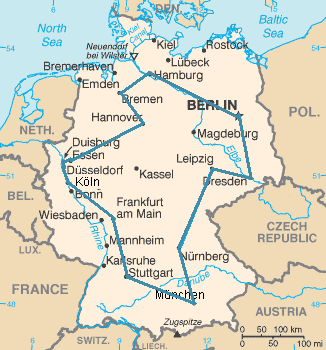
\includegraphics[width=0.8\textwidth]{TSP_Deutschland_3}
  \tiny

  user \textquote{Kapitän Nemo} \url{https://commons.wikimedia.org/w/index.php?curid=5584283}
\end{minipage}
\begin{minipage}{0.45\textwidth}

  \textquote{Given a list of cities and the distances between each pair of cities, what is the shortest possible route that visits each city exactly once and returns to the origin city?}
\cite{song_solving_2021}
\end{minipage}
\end{figure}

More formally the \ac{TSP} is defined as follows.
\begin{itemize}
  \item \textbf{Input}: A weighted (only non-negative weights), undirected, and complete graph.
  \item \textbf{Output}: A tour (cycle that visits every vertex) on the input graph, that uses each edge at most one time.
  \item \textbf{The optimization problem}: Find a valid output that has minimal (cumulative) edge weight.
\end{itemize}

For a more visual introduction to the problem, see the video essay ``The Traveling Salesman Problem: When Good Enough Beats Perfect'' by Reducible \cite{reducible_traveling_2022}.

\subsubsection{Why is TSP interesting?}

The \ac{TSP} is interesting for us, because of a few reasons.
First, the problem is well studied, thus good literature on the problem is easily found.
Then, the \ac{TSP} is known to be NP-hard, meaning that there can be found relatively small
input data, for which the solution takes large amounts of computing power, thus suggesting that \ac{HPC}
can be leveraged to speed up a computation.
Moreover, the problem is intuitive to understand and has practical applications in e.g. genome analysis,
satellite route planning, or fiber optical network design \cite{noauthor_tsp_2007},
using the 
\href{https://en.wikipedia.org/wiki/Concorde_TSP_Solver}{Concorde TSP Solver} software.

\subsubsection{The Implementation of this Project}
As a part of this project, a \ac{TSP} solver was implemented 
and made publicly available on GitHub\footnote{\url{https://github.com/lquenti/walky}},
the software has been built using the Rust programming language. 
To integrate into the Rust ecosystem, 
the solver has been published to crates.io as well\footnote{\url{https://crates.io/crates/walky/}}.
All the code is published and licensed under the permissive
\href{https://github.com/lquenti/walky/blob/main/LICENSE}{MIT open-source license} 
to encourage further third-party development.

\subsection{Goals and Contributions}

The following goals and contributions are defined for this project.

\begin{enumerate}
  \item Develop a CLI tool compatible with current state-of-the-art research
  \item Performance and Efficiency
    \begin{itemize}
      \item Create a blazingly fast software package
      \item Provide a 100\% pure Rust alternative to classical solvers
      \item Support both shared and distributed memory parallelization
      \item Achieve full documentation coverage
      \item Achieve high unit test coverage
    \end{itemize}
  \item Exact Solving
    \begin{itemize}
      \item Implement a simple, exact solver for the \ac{TSP}
      \item Offer several optimized versions
      \item Create a shared memory parallelized version
      \item Develop a distributed memory, parallelized solver based on \ac{MPI}
    \end{itemize}
  \item Approximation Tactics
    \begin{itemize}
      \item Include a trivial, easy-to-parallelize tactic and
      \item A sophisticated, state-of-the-art tactic
      \item For both:
        \begin{itemize}
          \item Provide a shared memory parallelized solver
          \item Provide a distributed memory, \ac{MPI}-based parallelized solver
        \end{itemize}
    \end{itemize}
  \item Lower Bound Calculation for \ac{TSP}
    \begin{itemize}
      \item Provide a sequential implementation
      \item Develop a parallelized implementation using \ac{MPI}
    \end{itemize}
\end{enumerate}
